\chapter{THS Compiler}
Der THS Compiler folgt dem theoretischen Aufbau eines Compilers und besteht aus Lexer, Parser und Code Generator. Als Parser wird ein Predictive Descent Parser verwendet.
Der Code Generator arbeitet auf dem Abstract Syntax Tree mithilfe eines Visitor Patterns. Die Semantic Analysis wird während der Code Generation durchgeführt. Geschrieben ist der Compiler in C++ und liefert x86 Assembly nach NASM Syntax.

\chapter{QHS Compiler}
Genauso wie der THS Compiler ist auch der QHS Compiler in C++ geschrieben und generiert x86 Assembly nach NASM Syntax.
Jedoch unterscheiden sich beide Compiler stark in der Funktionsweise. Der Compilation von QHS steht ein einfacher Zyklus zugrunde, dessen Vorbild der Von-Neumann Zyklus ist.

\begin{figure}[h!]
    \centering
    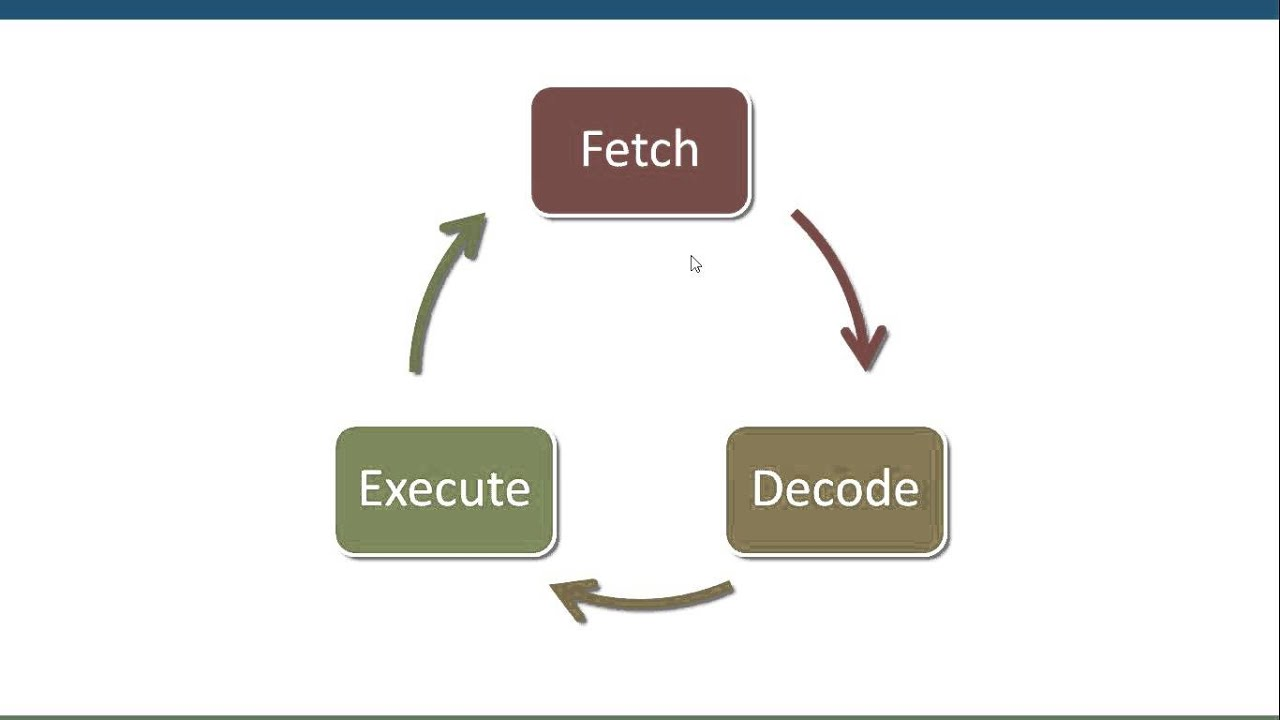
\includegraphics[scale=0.3]{resources/TEMP_von-neumann-cycle.jpg}
    \caption{TEMP! Zyklus der QHS Compilation, basierend auf Von-Neumann Zyklus}
    \label{fig:von-neumann-cycle}
\end{figure}

TALK ABOUT ORDERS AND THE MEANING OF IDENTIFIERS, INSTRUCTIONS AND LITERAL CODE

\section{Fetch} \label{sec:qhs-fetch}
Der QHS-Zyklus beginnt mit dem ersten Fetch. Dabei wird die erste Order aus dem Inputfile extrahiert. Eine Order weist einen der drei Typen Identifier, Instruction oder Literal-Code auf. Diese sind mit folgenden RegEx definiert.

\begin{table}[h]
    \centering
    \begin{tabular}{ll}
    \multicolumn{1}{l|}{identifier}        & \textless{}identiferChar\textgreater{}*                           \\ \hline
    \multicolumn{1}{l|}{instruction}       & \# \textless{}identiferChar\textgreater{}*                        \\ \hline
    \multicolumn{1}{l|}{literalCode}       & ".*"                                                              \\
                                           &                                                                   \\
    \textless{}identiferChar\textgreater{} & = {[}\textasciicircum{}\# "\textless{}whitespace\textgreater{}{]} \\
    \textless{}whitespace\textgreater{}    & = SPACE | NEWLINE | TAB
    
    \end{tabular}
\end{table}

Es ist hierbei möglich bestimmte Orders \textbf{voraus zu stellen}, die anstelle der nächsten Order im Inputfile gefetched werden. Dies geschieht mit Hilfe des Fetch-Stacks auf den eine Liste an Orders gepushed werden kann.
Dieser Fetch-Stack folgt Last-In First-Out und \textbf{auf ihn} kann während jeder der drei Schritte des Zyklus, meist jedoch während Execute, gepushed werden.
Die Hauptanwendung des Fetch-Stacks wird im Abschnitt \ref{sec:qhs-execute} ausgeführt.

\begin{figure}[h!]
    \centering
    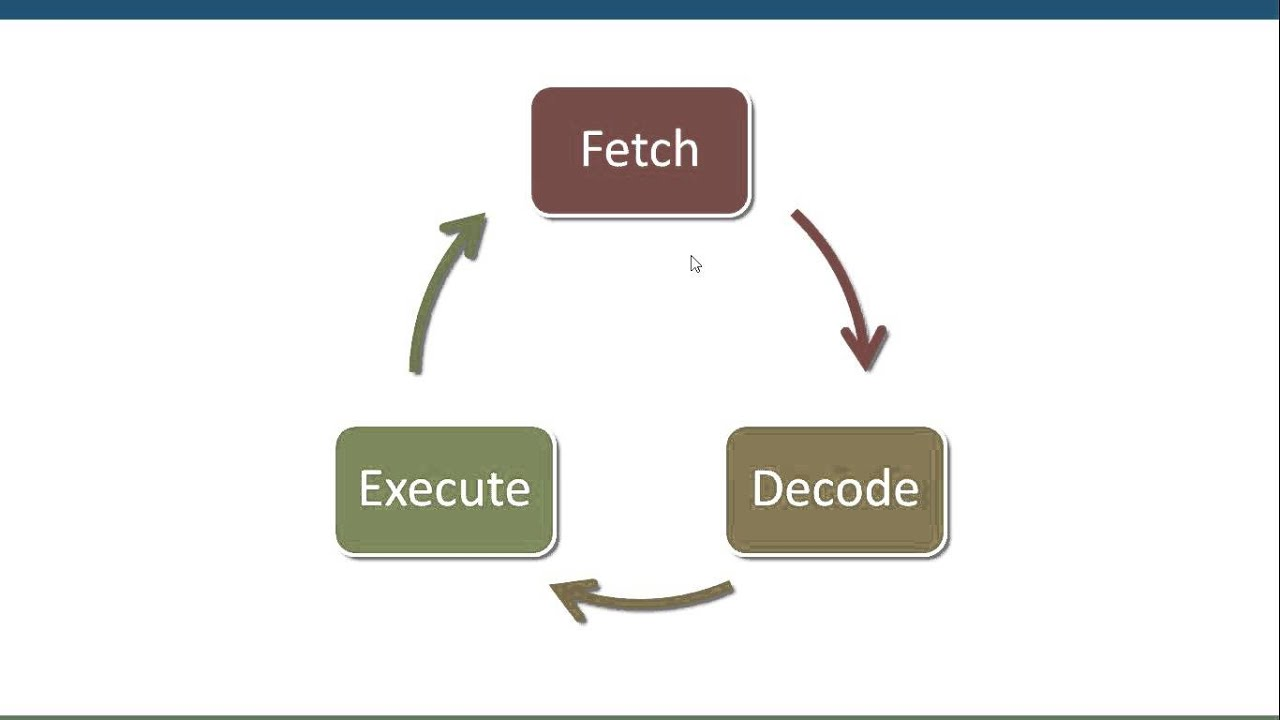
\includegraphics[scale=0.3]{resources/TEMP_von-neumann-cycle.jpg}
    \caption{TEMP! Struktur des Fetch-Stacks}
    \label{fig:fetch-stack}
\end{figure}

Wenn eine Liste an Orders komplett gefetched wurde, wird diese vom Stack gelöscht. Der Inputfile befindet sich auf dem letzten Platz des Fetch-Stacks und wird somit nur verwendet, wenn der Stack ansonsten komplett leer ist.
Die Compilation wird beendet, sobald keine Order mehr auf dem Fetch-Stack übrig ist.

\section{Decode} \label{sec:qhs-decode}
Nachdem eine Order gefetched wurde, wird diese an Decode weitergegeben. \textbf{Während Decode werden zwei Aufgaben durchgeführt}.

Während dem Decode Schritt kommt die Order-Queue ins Spiel. Hierbei handelt es sich um eine Liste an Orders, der Form First-In First-Out. Die Anwendung Aufgabe der Order-Queue ist das Speichern und spätere Ausführen von Orders.
Die Order-Queue kann mit Hilfe von Instructions, die im Abschnitt \ref{sec:qhs-execute} weiter ausgeführt werden, aktiviert und deaktiviert werden. Wenn nun eine Order in den Decode Schritt gelangt und die Order-Queue aktiviert ist,
wird diese Order der Order-Queue hinzugefügt. Der Execute Schritt wird danach übersprungen und der Zyklus beginnt von neuem bei Fetch. Die Order wurde ohne ausgeführt zu werden auf der Order-Queue gespeichert.
Später ist es nun möglich diese Order mit Hilfe von Instructions, die im Abschnitt \ref{sec:qhs-execute} weiter thematisiert werden, von der Order-Queue zu entfernen und auszuführen.
Bestimmte Instructions und Identifiers können jedoch Order-Queue-Proof, also immun gegen die Order-Queue, gemacht werden. Diese werden, auch wenn die Order-Queue aktiv ist, normal an Execute weitergegeben.
Dies ist zum Beispiel besonders bei der Instruction, die die Order-Queue wieder deaktiviert, wichtig. Da diese Instruction sonst nicht ausgeführt und somit die Order-Queue nie mehr deaktiviert wird.
LiteralCode kann nicht Code-Queue-Proof sein.

MAYBE CODESTACK FIGURE

Ist die Order-Queue deaktiviert oder die Order Code-Queue-Proof wird diese an den letzen Schritt Execute weitergegeben.

\section{Execute} \label{sec:qhs-execute}
Execute ist der letzte Schritt des Zyklus. Und hier wird nun auch endlich der tatsächliche Assembly Code generiert. Je nach Typ der Order, Identifier, Instruction oder Literal-Code, läuft Execute sehr unterschiedlich ab.

\subsection{Identifier}
Ein Identifier ist eine Zusammenfassung von mehreren Orders. Diese sind in einem Environment definiert. Hierbei handelt es sich um eine einfach Map (Dictionary), \textbf{die einen Identifier als string mit einer Liste an Orders verknüpft}.
Wenn nun ein Identifier in den Execute Schritt kommt, werden die dazugehörige Liste an Orders auf den Fetch-Stack aus Abschnitt \ref{sec:qhs-fetch} gepushed.
Beim nächsten Fetch werden nun die zum Identifier gehörenden Orders zurückgegeben. Um Grunde wird der Identifier mit seinen Orders ersetzt.

Environments sind hierbei in einer Linked-List gespeichert. Somit können neue Environments zu dieser Liste hinzugefügt und von der Liste entfernt werden. Das unterste Element der Liste ist hierbei das älteste und das oberste Element das neuste.
Bei der Definition eines Identifiers wird dieser immer zum obersten Environment hinzugefügt. Definitionen des gleichen Identifiers in älteren Environments werden nicht überschrieben oder gelöscht.
Bei der Abfrage nach einem Identifier wird immer die neuste vorhandene Definition zurückgegeben. Ist keine vorhanden wird ein Error ausgegeben.

\subsection{Literal-Code}
Literal-Code ist der Weg wie der QHS-Compiler Assembly Code generiert. Dieser ist sehr simpel. Wenn Literal-Code in den Execute Schritt gelangt, wird alles was zwischen den " Zeichen steht in das Output-Dokument geschrieben.

\subsection{Instructions}
Instructions sind die komplexeste Order für den Execute Schritt. Für jede Instruction ist im QHS-Compiler eine Funktion definiert, die ausgeführt wird, wenn diese Instruction in den Execute Schritt gelangt.
Diese Funktionen können Variabeln im QHS-Compiler speichern, den Order-Queue aktivieren, Identifier definieren und noch viel mehr. Folgend sind ein paar der wichtigsten Instructions aufgelistet.

\begin{table}[H]
    \centering
    \begin{tabularx}{\textwidth}{l|X}
    \textbf{\#enterOrderStack}   & Aktiviert die Order-Queue. \\ \hline
    \textbf{\#exitOrderStack}    & Deaktiviert die Order-Queue. \\ \hline
    \textbf{\#assignIdentifier}  & Das erste Element der Order-Queue muss ein Identifier sein. Der Rest der Orders auf Order-Queue wird als Definition für diesen Identifier festgelegt. \\ \hline
    \textbf{\#force}             & Die nächste Order wird nach Fetch sofort an Execute weitergegeben. Überspringt Decode und somit die Order-Queue. \\ \hline
    \textbf{\#orderEnqueue}      & Die nächste Order wird sofort der Order-Queue hinzugefügt, auch wenn diese Order Order-Queue-Proof wäre. Execute wird übersprungen. \\ \hline
    \textbf{\#orderFrontEnqueue} & Ähnlich wie \#orderEnqueue. Die Order wird jedoch auf den obersten Platz der Order-Queue gesetzt. \\ \hline
    \textbf{\#deepFetch}         & Wird mit der ersten Order der zweitobersten Liste an Order auf dem Fetch-Stack Ermöglicht den Zugriff auf den Inputfile innerhalb einer Identifier-Definition. \\ \hline
    \textbf{\#pushEnv}           & Ein neues Environment wird der Environment Linked-List hinzugefügt. \\ \hline
    \textbf{\#popEnv}            & Das neuste Environment der Environment Linked-List wird gelöscht.
        
    \end{tabularx}
\end{table}

Der QHScompiler umfässt \textbf{28} Instructions, wobei \textbf{5} dieser nur für Debugging des Compilers dienen.


